\documentclass[10pt,leqno]{jarticle}%スタイルの指定, titlepageを追加するとタイトルのページが独立
\usepackage{listings,jvlisting}
\pagestyle{plain}
\usepackage[dvipdfmx]{graphicx}
\usepackage{float}
\usepackage{url}

\lstset{
  basicstyle={\ttfamily},
  identifierstyle={\small},
  commentstyle={\smallitshape},
  keywordstyle={\small\bfseries},
  ndkeywordstyle={\small},
  stringstyle={\small\ttfamily},
  frame={tb},
  breaklines=true,
  columns=[l]{fullflexible},
  numbers=left,
  xrightmargin=0zw,
  xleftmargin=3zw,
  numberstyle={\scriptsize},
  stepnumber=1,
  numbersep=1zw,
  lineskip=-0.5ex
}

\begin{document} 
%この行は注釈。次の4行でタイトル、著者名、日付を表示する
\title{小レポート2} 
\author{3年 三田 周之介 \thanks{東京大学総合教育科学専攻教育社会科学専修比較教育社会学コース3年}} 
\date{2022年11月16日提出}  %期限:a月b日
\maketitle

\begin{description}
   \item[問1]\mbox{}\\
\textcircled{\scriptsize 1}
\begin{figure}[H]
  \centering
  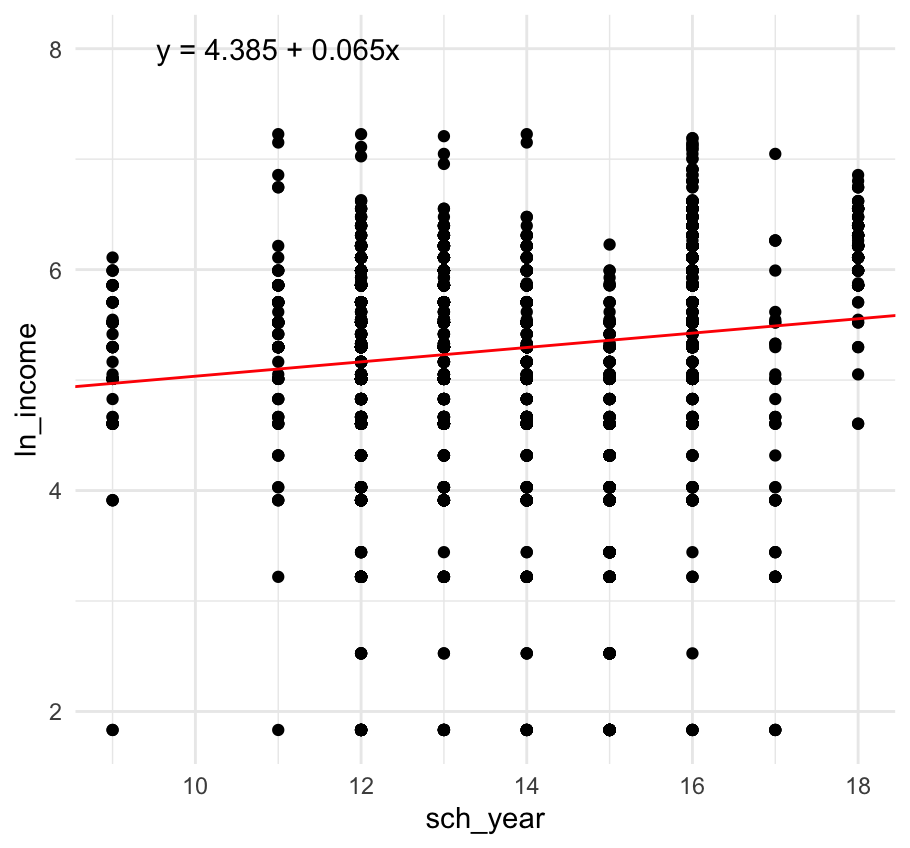
\includegraphics[width=10cm]{q1.png}
  \caption{従属変数が自然対数を取る時における, 独立変数と従属変数の散布図}
\end{figure}

\textcircled{\scriptsize 2} 
修学年度が1単位増加した時に自然対数をとった時の年収が6.5\%増加変化した

   \item[問2]\mbox{}\\
\textcircled{\scriptsize 1}
\begin{figure}[H]
  \centering
  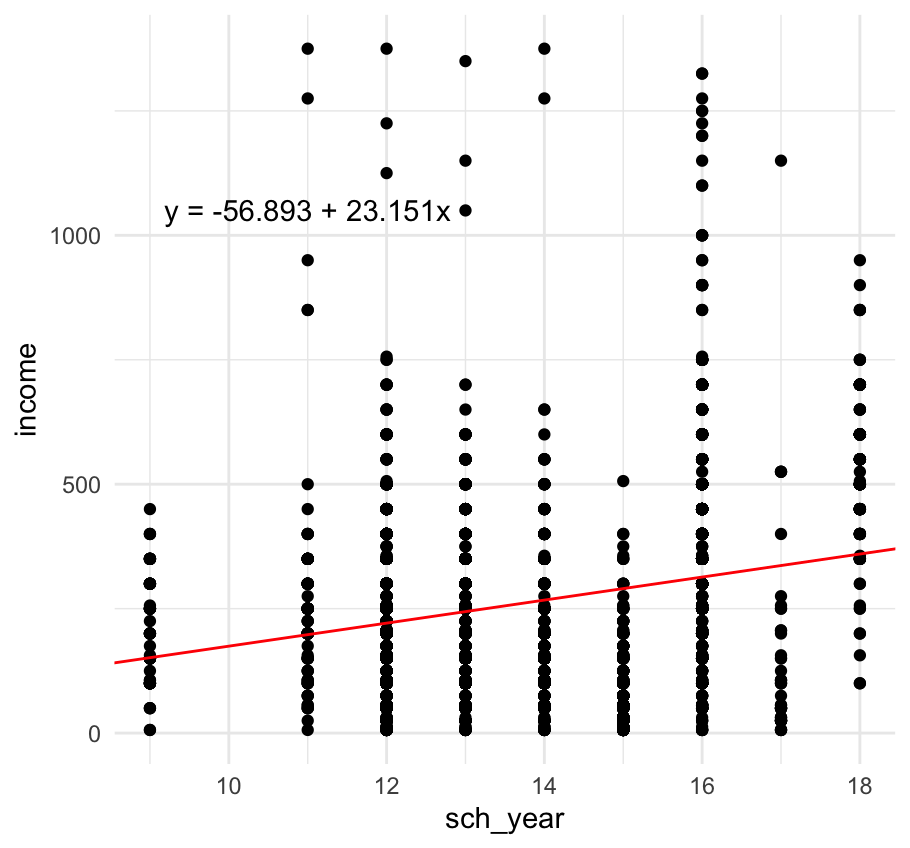
\includegraphics[width=10cm]{q2.png}
  \caption{従属変数が自然対数を取らない時における, 独立変数と従属変数の散布図}
\end{figure}

\textcircled{\scriptsize 2} 
修学年度が1単位増加した時に自然対数をとった時の年収が23.151単位増加変化した

\end{description}

\section*{[使用したコード]}
Rを用いた. 
なおtanaka2015.csvの内容については\url{https://github.com/MITA-Shunosuke/education-economics-3A-}を参照せよ.
\begin{lstlisting}[caption=使用したプログラム]
library(tidyverse)
library(ggpubr)
library(magrittr)
library(stargazer)
df <- read_csv("tanaka2015.csv")
sch_year <- df$修学年数 
ln_income <- df$`対数_年収(万円)`
income <- df$`年収(万円)`

fit <- lm(ln_income ~ sch_year, df)
stargazer(fit, type = "text", no.space = TRUE)
df %>% ggplot(aes(x = sch_year, y = ln_income)) +
  geom_point() +
  geom_abline(aes(intercept = 4.385, slope = 0.065), color="red") + 
  annotate(geom = "text", x = 11, y = 8, label = "y = 4.385 + 0.065x") + 
  theme_minimal()

fit2 <- lm(income ~ sch_year, df)
stargazer(fit2, type = "text", no.space = TRUE)
df %>% ggplot(aes(x = sch_year, y = income)) +
  geom_point() +
  geom_abline(aes(intercept = -56.893, slope =  23.151), color="red") + 
  annotate(geom = "text", x = 11, y = 1050, label = "y = -56.893 + 23.151x") + 
  theme_minimal()

\end{lstlisting}

\end{document} 



